\section{Third Member}
This is the section dedicated to one of the team members, and it should be written individually . It can include a range of things; first subsection is a space for you to point out the strengths and weaknesses of the module, including complaints about the module coordinator Max Wilson. The second section should have a selfie image with Max! The last part of it is the most important one. You will need to write a paragraph about what you have learned in this module. You can write it in \textbf{Bold} if you want or you can use other fonts. 

Please do not forget:
\begin{itemize}
	\item First paragraph should have your comments about the module
	\item Second one, a selfie img with Max
	\item Last one, what you learned in this module.
\end{itemize}

\subsection{Comments about the module}
The best parts of this module included working in a team which I found challenging yet fun at times.  I found that the lecture was well organised and well structured, however I found that the labs were stressful at times due to having such a limited period of time to complete the work in. 

\subsection{Selfie with Max}
\begin{figure}[h]
\caption{Selfie with Max}
\centering
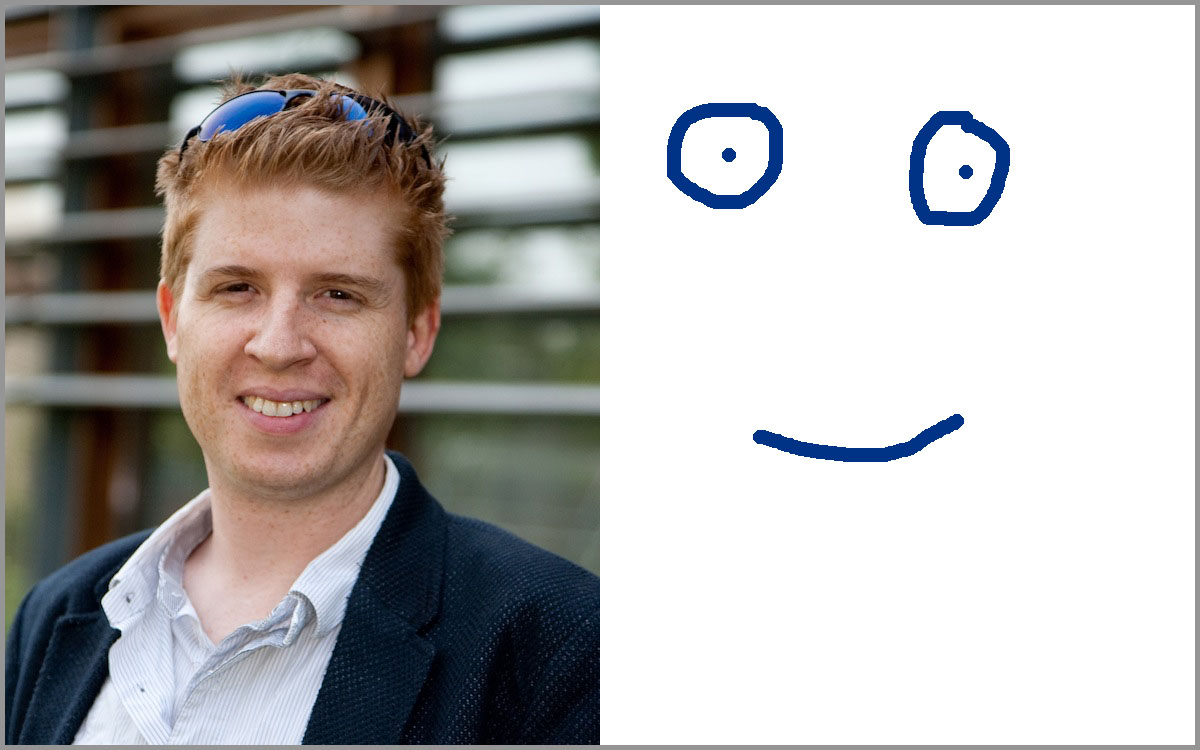
\includegraphics[width=0.5\textwidth]{imgWithMaxThird}
\label{fig:selfie}
\end{figure}

My selfie with Max is in Figure~\ref{fig:selfie}.

\subsection{What I have learned in this module}
In this module, I have learnt about the development cycle of software, along with agile development and the various testing and objective-gathering methods used in the process.

